\documentclass[12pt]{article}
\setlength{\oddsidemargin}{0in}
\setlength{\evensidemargin}{0in}
\setlength{\textwidth}{6.5in}
\setlength{\parindent}{0in}
\setlength{\parskip}{\baselineskip}
\usepackage{xcolor}

\usepackage{amsmath,amsfonts,amssymb}
\usepackage{graphicx}
\usepackage{enumitem}
\usepackage{fancyhdr}
\pagestyle{fancy}
\usepackage{hyperref}

\setlength{\headsep}{36pt}

\begin{document}

\lhead{{\bf CSCI 3104, Algorithms \\ Problem Set 10 -- Due Wed April 22 11:55pm} }
\rhead{Name: \fbox{\phantom{A really long name}} \\ ID: \fbox{\phantom{A reasonable ID}} \\ {\bf Profs.\ Chen \& Grochow \\ Spring 2020, CU-Boulder}}
\renewcommand{\headrulewidth}{0.5pt}

\phantom{Test}

\begin{small}
\textit{Advice 1}:\ For every problem in this class, you must justify your answer:\ show how you arrived at it and why it is correct. If there are assumptions you need to make along the way, state those clearly.

\vspace{-3mm} 
\textit{Advice 2}:\ Informal reasoning is typically insufficient for full credit. Instead, write a logical argument, in the style of a mathematical proof.

\textbf{Instructions for submitting your solutions}:
\vspace{-5mm} 

\begin{itemize}
	\item All submissions must be typed.
	\item You should submit your work through the \href{https://canvas.colorado.edu/courses/59906}{\textbf{class Canvas page}} only.
	\item You may not need a full page for your solutions; pagebreaks are there to help Gradescope automatically find where each problem is. Even if you do not attempt every problem, please allot at least as many pages per problem (or subproblem) as are allotted in this template.
%	\item For drawing graphs, you may include scans of hand-drawn graphs into your PDF file. \textbf{However, the rest of your solution (including the explanation of the graph) must be typed. If your words are not typed, you will get a 0 for that part of the question.}
\end{itemize}

Quicklinks: \ref{1a} \ref{1b} \ref{1c}  \ref{2a} \ref{2b}
\vspace{-4mm} 
\end{small}


\hrulefill

\newpage

\begin{enumerate}

\item \label{2} Consider the following DP table for the Knapsack problem for the list
\[
A = [(4, 3), (1, 2), (3, 1), (5, 4), (6, 3)]
\]

\noindent of (weight, value) pairs. The weight threshold $W = 10$.
\begin{itemize}
    \item Fill in the values of the table.
    \item Draw the backward path consisting of backward edges and do not draw (or erase them) the edges that are not part of the optimal backward paths.
\end{itemize}

\begin{enumerate}
    \item Fill the table with the above requirements (You can also re-create this table in excel/sheet).


\begin{figure}[h!]
\begin{center}
\includegraphics[scale=0.9]{DP_PS10.png}
\end{center}
\end{figure}
    \item Which cell has the optimal value and what is the optimal value for the given problem? \vskip 60pt
    
    \item List out the optimal subset and provide it's weight and value.
\end{enumerate}



\newpage 
\item Given the following directed acyclic graph. Use dynamic programming to fill in a table that counts number of paths from each node $j$ to 14, for $j \geq 1$. Note that a single vertex is considered a path of length $0$.

        % ----- FIGURE -----
        \begin{figure}[h!]
        \begin{center}
        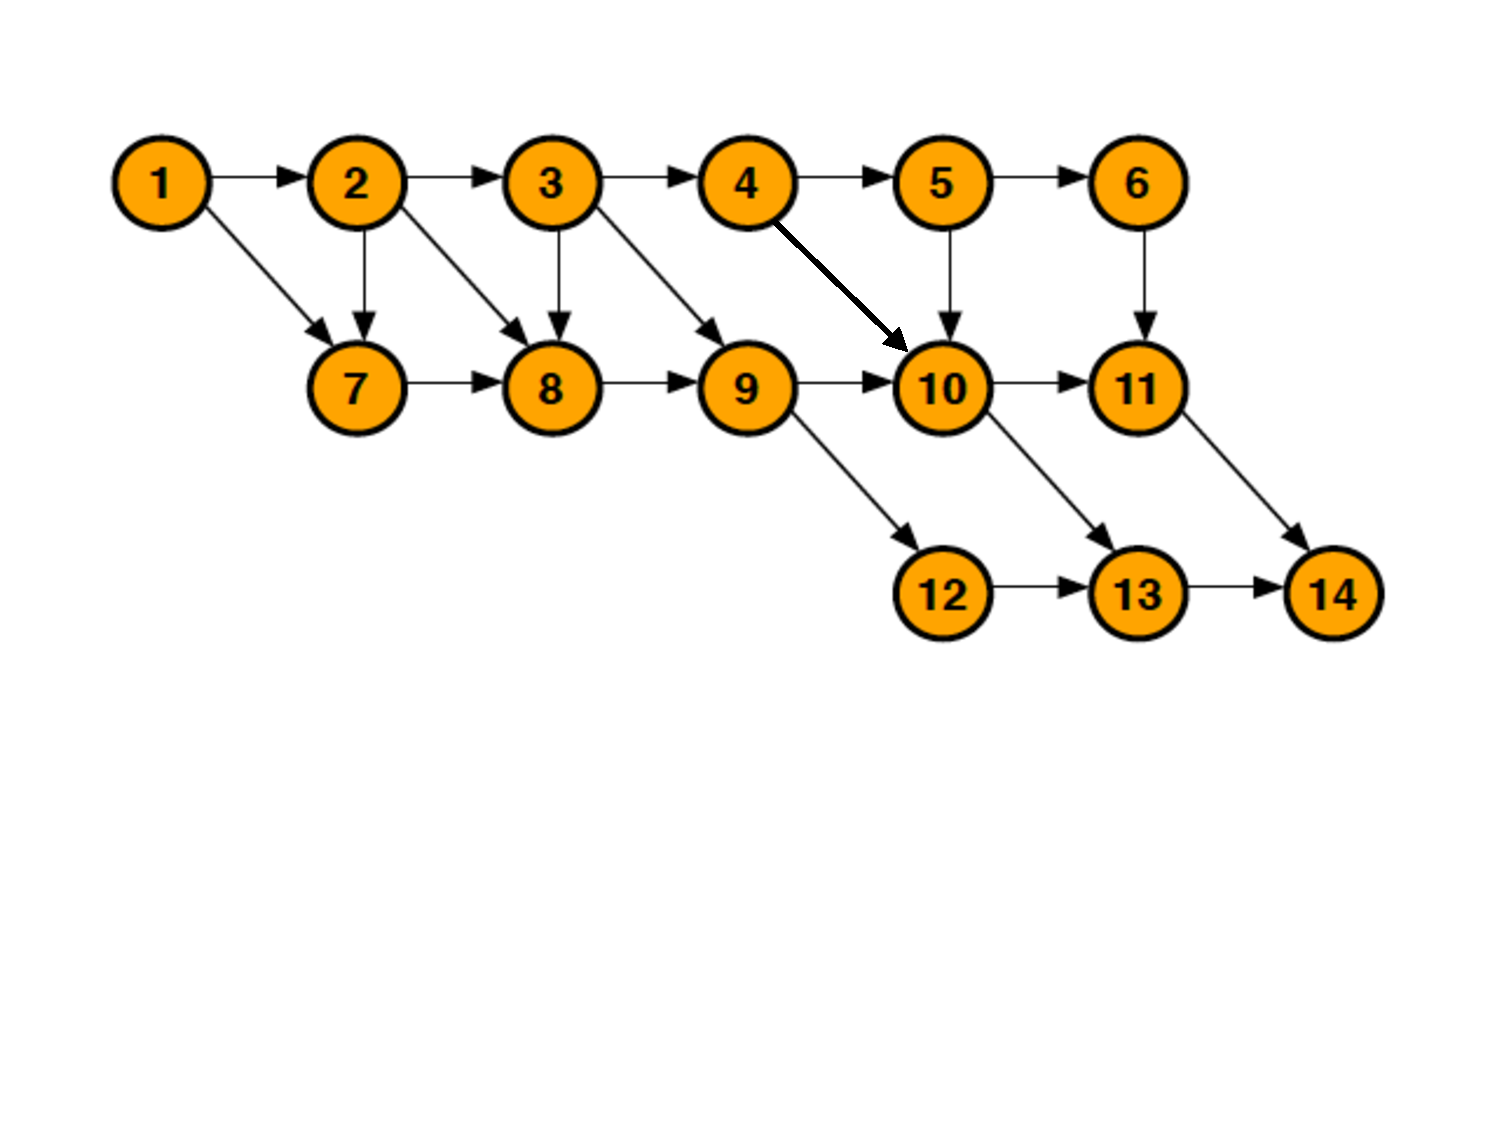
\includegraphics[scale=0.45]{dag_ps10.pdf} 
        \end{center}
        \end{figure}
        % ----------
\end{enumerate}
\end{document}


